%----------------------------------------------------------------------------------------
%	PACKAGES AND OTHER DOCUMENT CONFIGURATIONS
%----------------------------------------------------------------------------------------

\documentclass[a4paper,10pt,twoside]{article}
\usepackage[english]{babel}
\usepackage[utf8x]{inputenc}
\usepackage{amsmath}
\usepackage{graphicx}
\usepackage[colorinlistoftodos]{todonotes}
\usepackage{fancyhdr}
\usepackage[margin=0.73in]{geometry}

\setlength\paperheight{297mm}
\setlength\paperwidth{210mm}

\usepackage{avant}
\renewcommand{\familydefault}{\sfdefault}
\frenchspacing
 
\pagestyle{fancy}
\fancyhf{}
\fancyhead[LE,RO]{Mini Project Interim Report}
\fancyhead[RE,LO]{Adil \textsc{Bhayani} \& Sakayan \textsc{Sitsabesan}}
\fancyfoot[RE,LO]{\today}
\fancyfoot[LE,RO]{\thepage}
 
\renewcommand{\headrulewidth}{2pt}
\renewcommand{\footrulewidth}{1pt}

\begin{document}

\begin{titlepage}

\newcommand{\HRule}{\rule{\linewidth}{0.5mm}} % Defines a new command for the horizontal lines, change thickness here

\center % Center everything on the page
 
%----------------------------------------------------------------------------------------
%	HEADING SECTIONS
%----------------------------------------------------------------------------------------

\textsc{\LARGE University of Auckland}\\[1.5cm] % Name of your university/college
\textsc{\Large COMPSYS 305: Digital Systems Design 1}\\[0.5cm] % Major heading such as course name
\textsc{\large Mini Project }\\[0.5cm] % Minor heading such as course title

%----------------------------------------------------------------------------------------
%	TITLE SECTION
%----------------------------------------------------------------------------------------

\HRule \\[0.4cm]
{ \huge \bfseries Interim Report}\\[0.4cm] % Title of your document
\HRule \\[1.5cm]
 
%----------------------------------------------------------------------------------------
%	AUTHOR SECTION
%----------------------------------------------------------------------------------------

\begin{minipage}{0.4\textwidth}
\begin{flushleft} \large
\emph{Author:}\\
Adil \textsc{Bhayani} \newline
Sakayan \textsc{Sitsabesan}
\end{flushleft}
\end{minipage}
~
\begin{minipage}{0.4\textwidth}
\begin{flushright} \large
\emph{Supervisor:} \\
Dr. Muhammad \textsc{Nadeem} % Supervisor's Name
\end{flushright}
\end{minipage}\\[1cm]


%----------------------------------------------------------------------------------------
%	DATE SECTION
%----------------------------------------------------------------------------------------

{\large \today}\\[2cm] % Date, change the \today to a set date if you want to be precise

%----------------------------------------------------------------------------------------
%	LOGO SECTION
%----------------------------------------------------------------------------------------

\includegraphics{uoa.jpg}\\[1cm] % Include a department/university logo - this will require the graphicx package
 
%----------------------------------------------------------------------------------------

\vfill % Fill the rest of the page with whitespace

\end{titlepage}

\section{Design Overview}

The Mini Project consists of designing a game on a FPGA device which incorporates one simple tank defence game called Tank Hunting. The overall objective is to learn the process of digital design and logic by practically applying the skills learnt prior to the project.

\section{Design Specification}

\subsection{Available Equipment}

The following set of equipment has been provided for this project:

\begin{itemize}
\item DE0-Board
\item PS/2 Mouse
\item VGA Cable
\end{itemize}

\subsection{Design Definition and Requirements}

Tank Hunting is a simple 2D shooter game that revolves around controlling one tank to effectively destroy as many AI controlled tanks within a set time frame per level (game mode). The DE0 board which is acting as the console must interface with a monitor through a VGA cable to display a screen with a resolution of 640 x 480 pixels. The user will interface with the system through the DIP switches and buttons available on the board and through inputs from the PS/2 mouse.

The AI is to be designed so that it is bouncing on the edges of the screen in a horizontal line. The movement of the bottom tank is user controlled through the mouse and bullets can be shot by pressing the left mouse button. Both tanks must have two distinct colours. A bullet can only be shot when the other bullet has left the screen or when an AI tank has been hit. When a tank is hit, it must disappear and then reappear in a seemingly random x position while the player’s score should increase. Once all three levels have been cleared the game can be reset using the earlier mentioned buttons.

The levels should be designed in a manner which demonstrates increasing difficulty. This is achieved by increasing the speed of the AI controlled tanks and changing bullet speeds, alongside the implementation of additional features. 

\subsection{Optional Tasks and Additional Feature Design}

The first AI tank will be given the ability to shoot back at the player’s tank. If the players tank is hit then the game will end. Additionally, a secondary tank is to be added which will begin to move down towards the player. The game will also end if the tank goes off the screen or collides with the player’s tank. 

The set of requirements listed above are essential minimums and form a general guideline for the design of the system. To improve gameplay and to make the game more challenging additional features are to be implemented and incorporated in a manner which allows the game to flow and become increasingly difficult as levels are cleared. These will be discussed in greater detail in game strategy.

\section{Block Diagram}

\quad\:\:\:\textbf{LSFR:} The LSFR generates a random seed for the starting location of AI tanks. The output is a eleven bit number.

\textbf{Mouse:} Manages all signals sent to and from the mouse. The mouse column data and the button click data is passed on to the Tank entity which process the data.

\textbf{Clock Divider:} Divides the 50Mhz clock signal down to 1Hz for the counter to count in seconds.

\textbf{Counter:} Countdown timer for the game levels to time the lenght of the levels. Output is passed for rendering by Game Text entity.

\textbf{Char ROM:} Stores the pixel information for rendering text in the game. Accessed by the Game Text entity.

\textbf{Game Text:} Generates the appropriate text for the current screen and passes the output to the game entity for it to be muxed into the VGA signal.

\textbf{Tank:} The Tank entity to control movement, shooting and score of tanks. Inputs from mouse, LSFR \& game. Outputs the score to the Seven segment decoder and game text aas well as outputing the RGB signals to the game entity.

\textbf{Seven Segment Decoder:} Decodes the scores and mouse column packet data and outputs it to the seven segment decoder.

\textbf{Game:} Manages the game scene to render and muxes in the appropriate signals from the game text and tank entities. Uses an FSM to manage game state.

\textbf{VGA\_Sync:} Syncs the VGA signal to be sent out of the VGA port to the monitor. VGA sync signals are looped back to the Game Text and Tank entity for alligning the pixels on the screen.

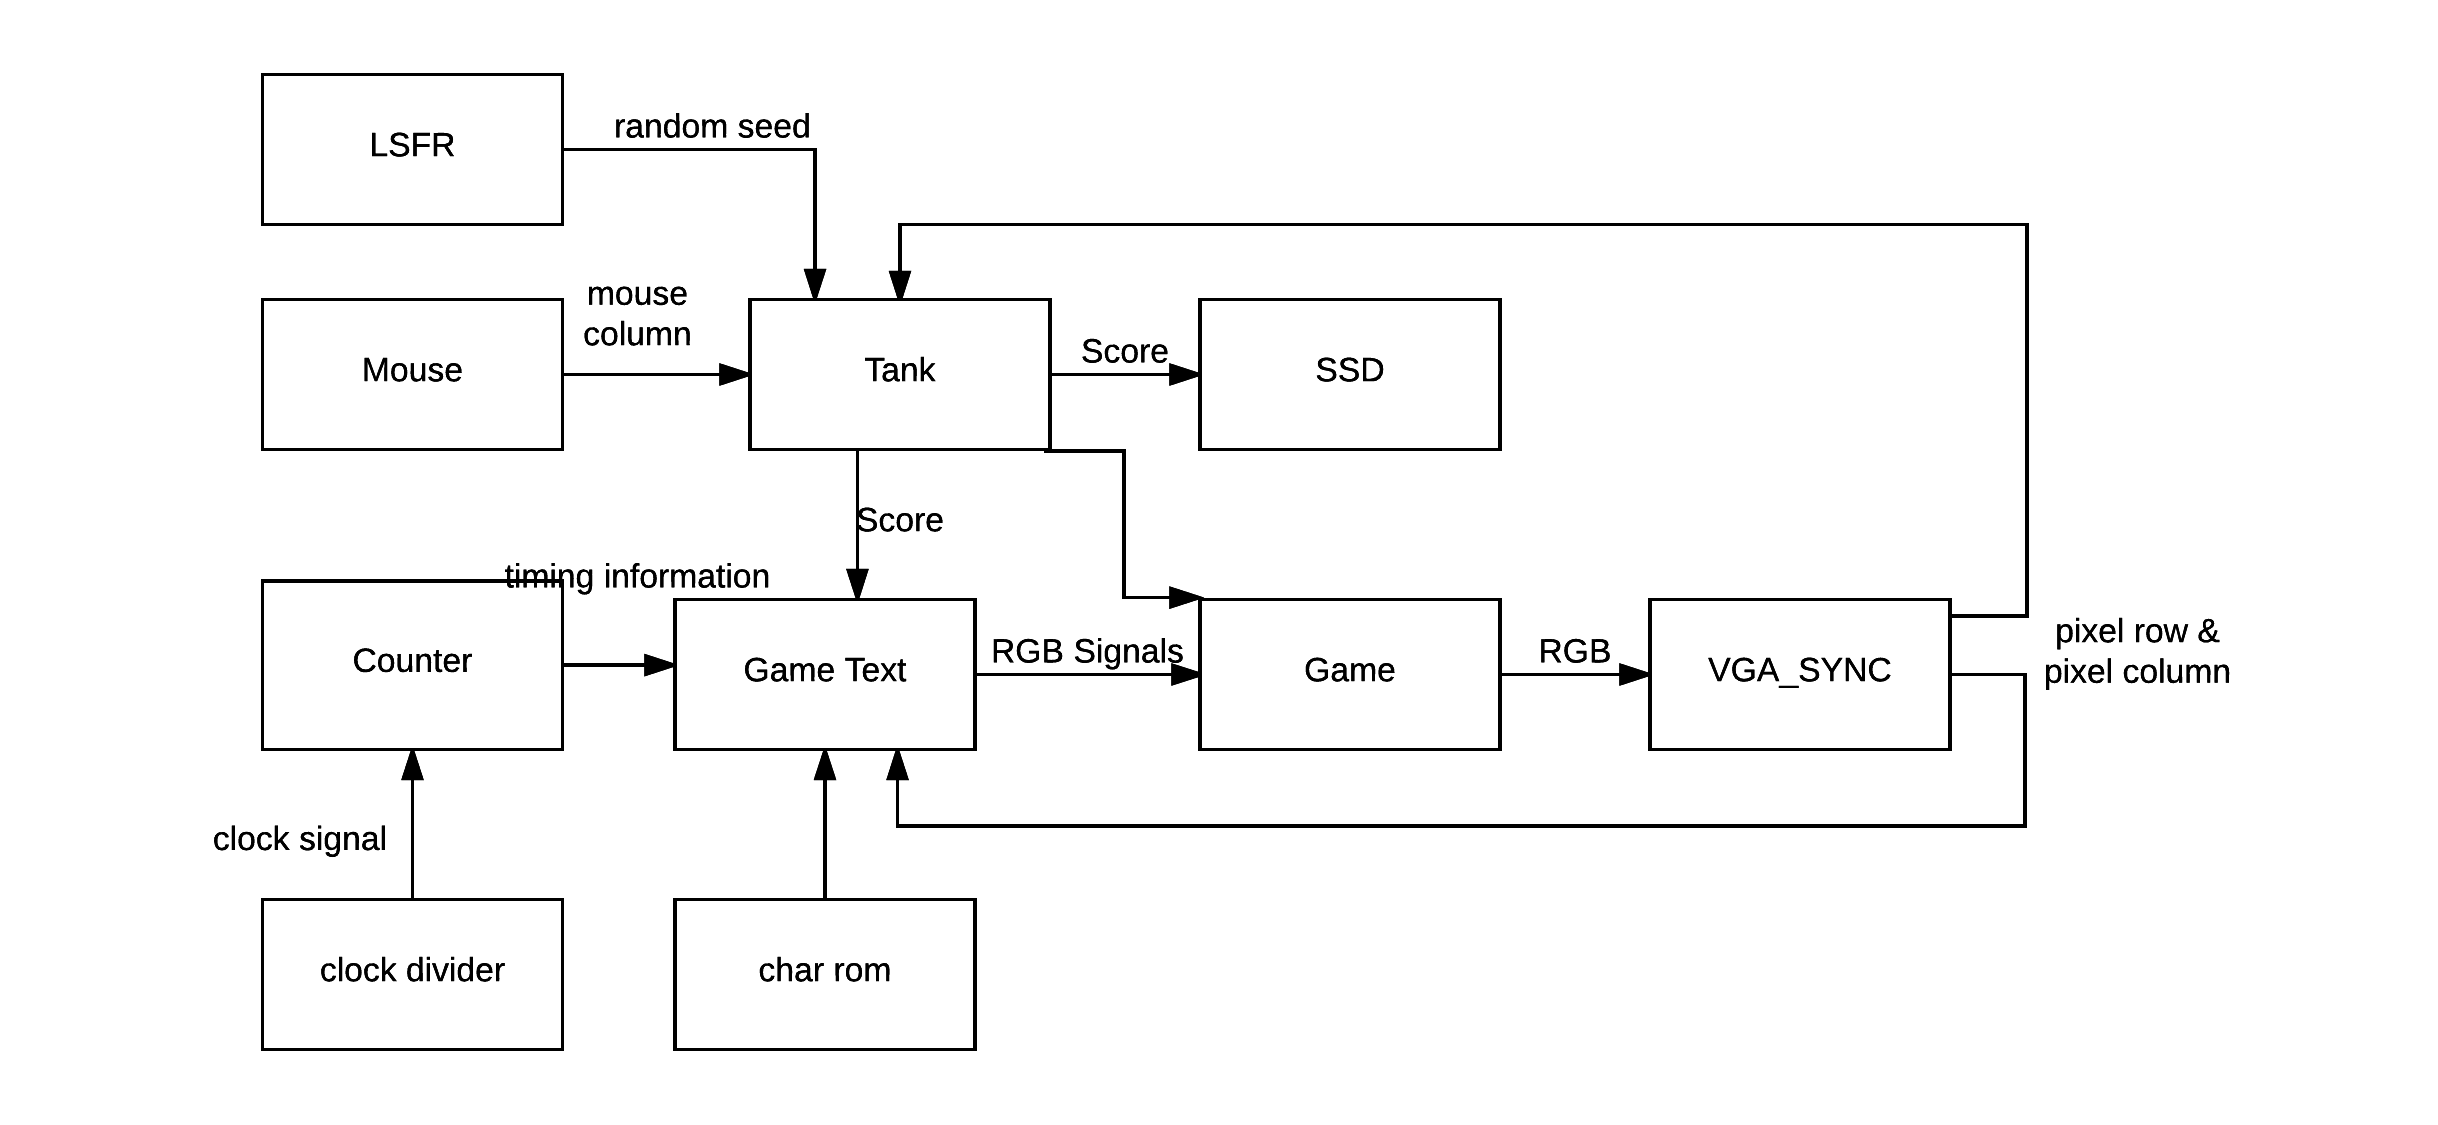
\includegraphics[width=1\textwidth]{block_diagram.png}

\section{Game Strategy}

The main objective of the game is to complete all three levels without losing as well as to get the highest score possible. Since the game will consist of three levels that will be of increasing difficulty, transitions will happen after the specified time has been reached. This allows the player to maximise their score by playing until the time limit has been reached. Once a level has been cleared the player's score will be shown on the screen as an intermediate progress screen, which can also be customised to incorporate a story. By interacting with the push buttons the player can continue to the next level. The score will be retained across all levels allowing the player to accumulate their score and aim for a new high score.

\subsection{Level 1}

The first level will only have one AI controlled tank that will move slowly across the top of the screen. The player will be able to move across the screen faster than the AI and can easily score many points considering the bullet speed is also very high.

\subsection{Level 2}

This level brings in the addition of the second tank and increases the speed of both AI tanks. The user’s tank speed remains unchanged to increase the difficulty. A restriction will be placed on the number of bullets that the user can shoot, with the ability to get back bullets by successfully hitting an AI tank.

\subsection{Level 3}

The final level of the game will be designed to be truly challenging. Alongside the increased AI tank speed, one tank will now move downwards towards the player’s tank while the other will shoot back at the player. If a bullet hits the player the game will immediately end. Similarly, collisions between the downward moving AI tank and the player’s tank or the AI tank moving off the screen downwards will also cause the game to end. This means that the player will now have to actively defend him/herself while attempting to increase their score. Bullet restrictions will remain, similar to level two. 

\section{Appendices}

\subsection{Extended Block Diagrams}

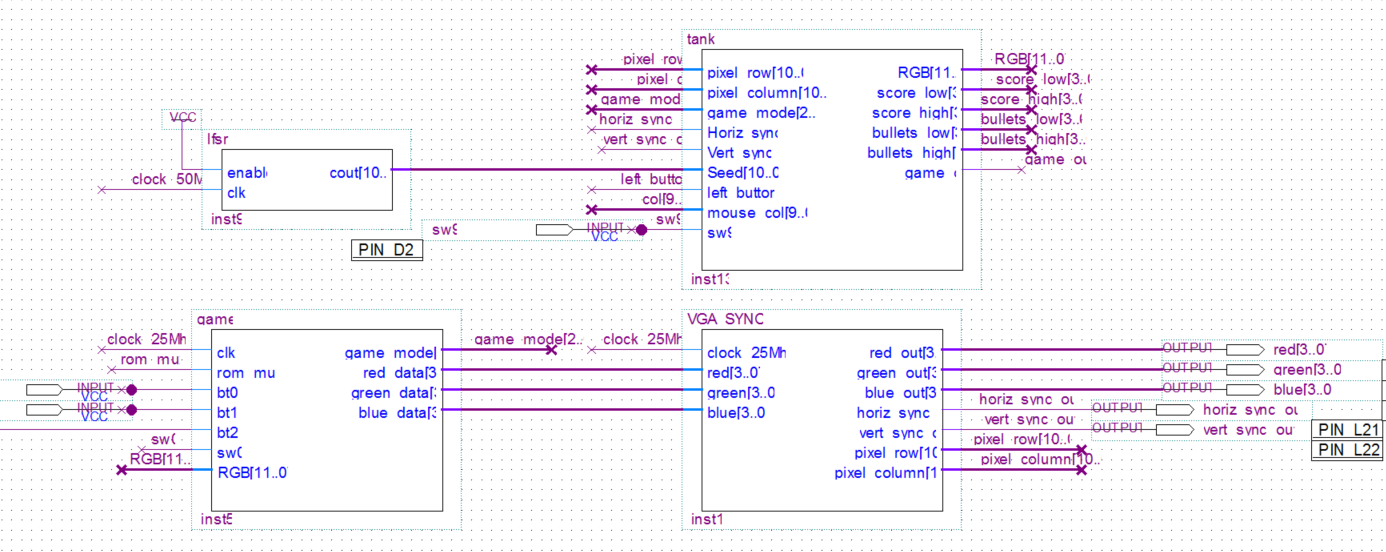
\includegraphics[width=1\textwidth]{appendix1.png}

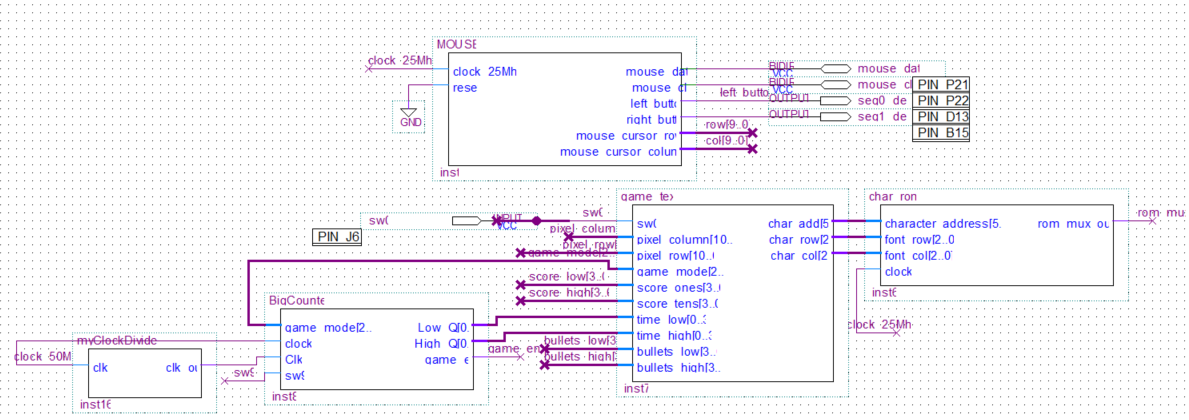
\includegraphics[width=1\textwidth]{appendix2.png}

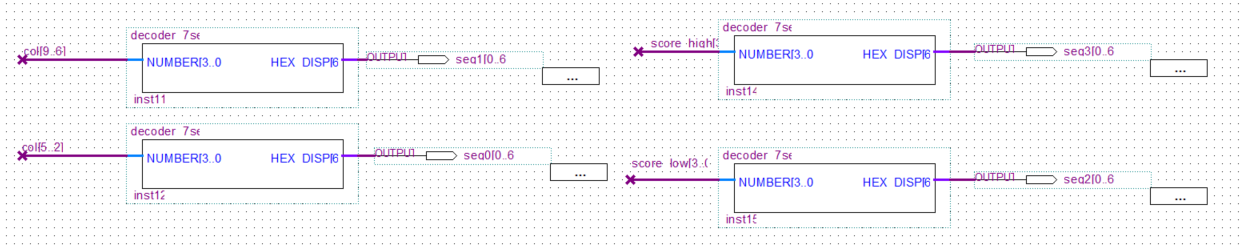
\includegraphics[width=1\textwidth]{appendix3.png}

\end{document}